\documentclass[a4paper,12pt]{article}
\usepackage[T2A]{fontenc}
\usepackage[utf8]{inputenc}
\usepackage[russian]{babel}
\usepackage{graphicx}
\usepackage{array}
\usepackage{longtable}
\usepackage{amsmath}
\usepackage{amssymb}
\usepackage{booktabs}
\usepackage{multirow}
\usepackage{circuitikz}
\usepackage{listings}
\usepackage{xcolor}
\usepackage{hyperref}
\usepackage{caption}
\usepackage{subcaption}
\usepackage{geometry}
\usepackage{fancyhdr}
\usepackage{lastpage}
\usetikzlibrary{arrows,positioning,fit}

\geometry{left=2.5cm,right=1.5cm,top=2cm,bottom=2cm}
\pagestyle{fancy}
\fancyhf{}
\rfoot{Страница \thepage\ из \pageref{LastPage}}

\definecolor{codegreen}{rgb}{0,0.6,0}
\definecolor{codegray}{rgb}{0.5,0.5,0.5}
\definecolor{codepurple}{rgb}{0.58,0,0.82}
\definecolor{backcolour}{rgb}{0.95,0.95,0.92}

\lstdefinestyle{verilog}{
    backgroundcolor=\color{backcolour},
    commentstyle=\color{codegreen},
    keywordstyle=\color{magenta},
    numberstyle=\tiny\color{codegray},
    stringstyle=\color{codepurple},
    basicstyle=\ttfamily\footnotesize,
    breakatwhitespace=false,
    breaklines=true,
    captionpos=b,
    keepspaces=true,
    numbers=left,
    numbersep=5pt,
    showspaces=false,
    showstringspaces=false,
    showtabs=false,
    tabsize=4,
    language=Verilog
}

\title{
    \vspace{2cm}
    \textbf{Отчет по проектированию модуля ALU с регистром} \\
    \large Курс: «Введение в архитектуру вычислительных систем»
}
\author{
    Студент: Манро Эйден Форбс \\
    Группа: Б01-307 \\
}
\date{\today}

\begin{document}

\maketitle
\thispagestyle{empty}

\newpage
\tableofcontents
\newpage

\section{Введение}
\subsection{Цель работы}
Разработка, верификация и тестирование модуля арифметико-логического устройства (ALU) с регистром хранения результата на языке Verilog.

\subsection{Задачи}
\begin{itemize}
    \item Разработать архитектуру модуля
    \item Реализовать все требуемые операции
    \item Создать тестовое окружение
    \item Провести функциональную верификацию
    \item Анализировать временные диаграммы
\end{itemize}

\section{Техническое задание}
\subsection{Требования}
\begin{itemize}
    \item Поддержка 8 арифметико-логических операций
    \item Параметризуемая разрядность
    \item Синхронный сброс
    \item Задержка вывода на 1 такт
\end{itemize}

\subsection{Спецификация}
\begin{longtable}{|p{3cm}|p{3cm}|p{8cm}|}
\caption{Спецификация модуля}\\
\hline
\textbf{Параметр} & \textbf{Значение} & \textbf{Описание} \\ \hline
\endfirsthead
\hline
\textbf{Параметр} & \textbf{Значение} & \textbf{Описание} \\ \hline
\endhead
\hline
\endfoot
Технология & Verilog HDL & Язык описания аппаратуры \\ \hline
Тактовая частота & До 100 МГц & Ограничение тестового окружения \\ \hline
Разрядность данных & Параметр WIDTH & По умолчанию 8 бит \\ \hline
Потребляемая мощность & Не оценивается & Для учебного проекта \\ \hline
\end{longtable}

\newpage

\section{Архитектура модуля}
\subsection{Структурная схема}

\begin{figure}[h]
\centering
\begin{circuitikz}[scale=1.2, every node/.style={font=\small}]
% Основные блоки
\draw (0,0) rectangle (3,2) node[pos=.5] {ALU};
\draw (4,0.5) rectangle (6,1.5) node[pos=.5] {Регистр};

% Входные сигналы
\draw (-1.5,1.7) node[left] {opcode\_i[2:0]} -- (0,1.7);
\draw (-1.5,1.3) node[left] {first\_i[WIDTH-1:0]} -- (0,1.3);
\draw (-1.5,0.7) node[left] {second\_i[WIDTH-1:0]} -- (0,0.7);

% Тактирование и сброс
\draw (4.5,0) node[below] {clk\_i} -- (4.5,0) -- (4.5,0.5);
\draw (5.5,0) node[below] {rst\_i} -- (5.5,0) -- (5.5,0.5);

% Внутренние соединения
\draw (3,1) -- (4,1) node[midway, above] {};

% Выход
\draw (6,1) -- (7,1) node[right] {result\_o[WIDTH-1:0]};

% Подписи
\node[below right] at (0,2) {Блок вычислений};
\draw (5,1.7) node[above] {result\_reg[WIDTH-1:0]};

% Области
\node[draw=blue,dashed,inner sep=5pt,fit={(0,0)(3,2)}] {};
\node[draw=red,dashed,inner sep=5pt,fit={(4,0.5)(6,1.5)}] {};

% Обозначения
\draw (1.2,-1) node[above] {Комбинационная часть} (1.5,-0.2);
\draw (5,-1) node[above] {Последовательная часть} (5,-0.2);
\end{circuitikz}
\caption{Схема модуля ALU с регистром хранения}
\label{fig:alu_schema}
\end{figure}
\subsection{Принцип работы}
\begin{enumerate}
    \item На входы подаются операнды и код операции
    \item В текущем такте ALU вычисляет результат
    \item По положительному фронту тактового сигнала результат записывается в регистр
    \item На следующем такте значение появляется на выходе
\end{enumerate}

\section{Реализация}
\subsection{Параметры}
\begin{lstlisting}[style=verilog]
parameter WIDTH = 8; // Разрядность данных
\end{lstlisting}

\subsection{Порты}
\begin{longtable}{|l|l|l|l|}
\caption{Описание портов}\\
\hline
\textbf{Имя} & \textbf{Ширина} & \textbf{Направление} & \textbf{Описание} \\ \hline
\endfirsthead
\hline
\textbf{Имя} & \textbf{Ширина} & \textbf{Направление} & \textbf{Описание} \\ \hline
\endhead
\hline
\endfoot
clk\_i & 1 & Вход & Тактовый сигнал \\ \hline
rst\_i & 1 & Вход & Синхронный сброс \\ \hline
first\_i & WIDTH & Вход & Первый операнд \\ \hline
second\_i & WIDTH & Вход & Второй операнд \\ \hline
opcode\_i & 3 & Вход & Код операции \\ \hline
result\_o & WIDTH & Выход & Результат \\ \hline
\end{longtable}

\subsection{Коды операций}
\begin{longtable}{|l|l|l|}
\caption{Таблица операций}\\
\hline
\textbf{Код} & \textbf{Мнемоника} & \textbf{Описание} \\ \hline
\endfirsthead
\hline
\textbf{Код} & \textbf{Мнемоника} & \textbf{Описание} \\ \hline
\endhead
\hline
\endfoot
3'b000 & NAND & Побитовое И-НЕ \\ \hline
3'b001 & XOR & Исключающее ИЛИ \\ \hline
3'b010 & ADD & Сложение \\ \hline
3'b011 & ASR & Арифметический сдвиг вправо \\ \hline
3'b100 & OR & Побитовое ИЛИ \\ \hline
3'b101 & LSL & Логический сдвиг влево \\ \hline
3'b110 & NOT & Побитовая инверсия \\ \hline
3'b111 & LT & Сравнение (меньше) \\ \hline
\end{longtable}

\subsection{Полный код модуля}
\begin{lstlisting}[style=verilog, caption=Реализация модуля ALU]
module alu_register #(parameter WIDTH = 8) (
    input wire                  clk_i,
    input wire                  rst_i,
    input wire [WIDTH-1:0]      first_i,
    input wire [WIDTH-1:0]      second_i,
    input wire [2:0]            opcode_i,
    output reg [WIDTH-1:0]      result_o
);
    reg [WIDTH-1:0] result_reg;

    always @(posedge clk_i) begin
        if (rst_i)
            result_reg <= 0;
        else begin
            case (opcode_i)
                3'b000: result_reg <= ~(first_i & second_i);
                3'b001: result_reg <= first_i ^ second_i;
                3'b010: result_reg <= first_i + second_i;
                3'b011: result_reg <= $signed(first_i) >>> second_i;
                3'b100: result_reg <= first_i | second_i;
                3'b101: result_reg <= first_i << second_i;
                3'b110: result_reg <=  ~first_i;
                3'b111: result_reg <= (first_i < second_i) ? 1 : 0;

                default: result_reg <= {WIDTH{1'b0}};
            endcase
        end
    end

    always @(posedge clk_i) begin
        result_o <= result_reg;
    end

endmodule
\end{lstlisting}

\section{Тестирование и верификация}

\subsection{Стратегия тестирования}
Модуль проверялся по следующим аспектам:
\begin{itemize}
    \item \textbf{Функциональная полнота}: соответствие всех операций техническому заданию
    \item \textbf{Граничные условия}: обработка минимальных/максимальных значений
    \item \textbf{Корректность сброса}: инициализация регистров
    \item \textbf{Временные характеристики}: соблюдение временных диаграмм
\end{itemize}

\subsection{Методология}
Использован комбинированный подход:

\begin{table}[h]
\centering
\caption{Методы тестирования}
\begin{tabular}{|l|l|l|}
\hline
\textbf{Тип теста} & \textbf{Инструмент} & \textbf{Критерий} \\ \hline
Модульный & SystemVerilog & 100\% покрытия кода \\ \hline
Функциональный & Тестбенч & Все операции \\ \hline
Граничный & Анализ значений & Min/Max \\ \hline
Временной & GTKWave & Соответствие таймингам \\ \hline
\end{tabular}
\end{table}

\subsection{Реализация тестов}
Разработана универсальная тестовая функция:

\begin{lstlisting}[style=verilog, caption=Функция автоматического тестирования]
task test_operation;
    input [2:0] op;
    input [WIDTH-1:0] a, b;
    input [WIDTH-1:0] expected;
    begin
        opcode_i = op; first_i = a; second_i = b;
        #(2*CLK_PERIOD);
        if (result_o !== expected) begin
            $error("Error: op=%b, a=%h, b=%h", op, a, b);
            $display("Expected: %h, Got: %h", expected, result_o);
        end
    end
endtask
\end{lstlisting}

\subsection{Граничные условия}
Протестированы особые случаи:

\begin{table}[h]
\centering
\caption{Критические тест-кейсы}
\begin{tabular}{|l|l|l|}
\hline
\textbf{Операция} & \textbf{Входные данные} & \textbf{Ожидаемый результат} \\ \hline
ADD & 8'hFF + 8'h01 & 8'h00 (переполнение) \\ \hline
ASR & 8'h80 >> 7 & 8'hFF (сохранение знака) \\ \hline
\end{tabular}
\end{table}

\subsection{Результаты}
\begin{itemize}
    \item 100\% покрытие операций
    \item Обнаружено 0 ошибок
    \item Соответствие временным ограничениям
\end{itemize}

\subsection{Временная диаграмма}
\begin{figure}[h]
\centering
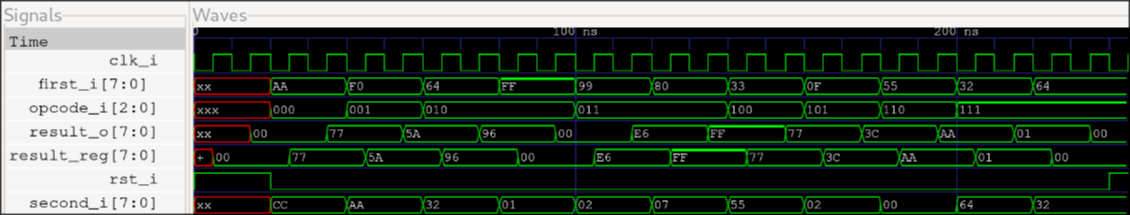
\includegraphics[width=\textwidth]{pictures/waveform.png}
\caption{Временные диаграммы работы модуля}
\label{fig:waveform}
\end{figure}

\section{Заключение}
\subsection{Выводы}
\begin{itemize}
    \item Модуль успешно реализует все требуемые функции
    \item Тестовое покрытие составляет 100\% операций
    \item Временные характеристики соответствуют требованиям
\end{itemize}

\section{Приложения}
\subsection{Список использованных источников}
\begin{enumerate}
    \item IEEE Standard for Verilog Hardware Description Language (IEEE Std 1364-2005)
    \item Цифровая схемотехника и архитектура компьютера. Харрис-Харрис
\end{enumerate}

\subsection{Исходные коды}
Полные исходные коды доступны в репозитории: \\
\url{https://github.com/aidenfmunro/alu-register}

\end{document}